%%%%%%%%%%%%%%%%%%%%%%%%%%%%%%%%%%%%%%%%%
% University/School Laboratory Report
% LaTeX Template
% Version 3.0 (4/2/13)
%
% This template has been downloaded from:
% http://www.LaTeXTemplates.com
%
% Original author:
% Linux and Unix Users Group at Virginia Tech Wiki 
% (https://vtluug.org/wiki/Example_LaTeX_chem_lab_report)
%
% License:
% CC BY-NC-SA 3.0 (http://creativecommons.org/licenses/by-nc-sa/3.0/)
%
%%%%%%%%%%%%%%%%%%%%%%%%%%%%%%%%%%%%%%%%%

%----------------------------------------------------------------------------------------
%  PACKAGES AND DOCUMENT CONFIGURATIONS
%----------------------------------------------------------------------------------------

\documentclass{article}

\usepackage{siunitx} % Provides the \SI{}{} command for typesetting SI units

\usepackage{graphicx} % Required for the inclusion of images
\usepackage{caption}
\usepackage{subcaption}
\usepackage{geometry}
\usepackage{float}
\usepackage{amsmath, amssymb}
\usepackage{mathtools}
\usepackage[usenames,dvipsnames,table]{xcolor}
\setlength\parindent{0pt} % Removes all indentation from paragraphs

%\renewcommand{\labelenumi}{\alph{enumi}.} % Make numbering in the enumerate environment by letter rather than number (e.g. section 6)

%\usepackage{times} % Uncomment to use the Times New Roman font
\geometry{hmargin=2cm,vmargin=2cm}

%----------------------------------------------------------------------------------------
%  DOCUMENT INFORMATION
%----------------------------------------------------------------------------------------

\title{Assignement 1 \\ High Performance Scientific Computing} % Title

\author{Pierre \textsc{Lorent} -- Damien \textsc{Smeets}} % Author name

\date{\today} % Date for the report

\definecolor{light-gray}{gray}{0.95}
\definecolor{extra-gray}{gray}{0.75}
\definecolor{medium-gray}{gray}{0.85}

\begin{document}

\maketitle % Insert the title, author and date

\begin{center}
\begin{tabular}{l r}
Instructor: & Professor \textsc{Geuzaine}\\ % Instructor/supervisor
Assistant: & Amaury \textsc{Johnen}
\end{tabular}
\end{center}

\section*{Implementation}
We organized the code in two parts: the main computation unit and a library allowing to perform basic vector operations. This choice may induce some additionnal operations during computation but avoids the introduction of redundancy into the code, thus making it easier to read and to verify the formulae.\\

As the equations given are rather simple and imply a small number of variables, the computation only requires one loop to iterate and compute the new positions depending on the 2 previous positions and the current speed.\\

As the step interval and the output interval may be different, we also take into account the case where outputs are asked at a time where no data is available. In this particular case, the previous data is provided whith the computation time. Example: with \texttt{(dt, dt\_out) = (1, 4.5)}, we will have an output of the position at \texttt{[0, 4, 9, 13, 18]}.


\subsection*{Additional features}
After the implementation of the required functionalities, we decided to add some interesting features to allow a deeper analysis of the computed data. The final version of the code includes two options:
\begin{itemize}
\item \texttt{-v} launches the program in verbose mode.
\item \texttt{-m} allows to specify a secondary output file to produce a \textsc{Matlab} file with the results. This allows to have a visual feedback on the global evolution of the positions.
\end{itemize}

The extended syntax to use these features is:\\
\texttt{./a.out input.dat output.dat [-v] [-m <filename>]}


\section*{Results}
We first tried our implementation with real-life parameters: the Earth around the Sun (shown on Fig. \ref{fig:earthsun}), a geostationnary satellite around the Earth (shown on Fig. \ref{fig:satgeo}) and an example of Newton's Cannon (on Fig. \ref{fig:nc}).\\

Then we tried to find parameters that could model a binary star system (which is called the two-body problem). We did eventually find something that looks like a binary star system, but the two stars are much too close from each other, and it's spinning way too fast. However, it gives some interesting insight on how it can work (we put \texttt{z} axis velocities as well for fun and experimentation). It will also give us the opportunity to discuss the method's limits: the $\Delta t$ here becomes very relevant. Figure \ref{fig:sample} shows the same initial conditions, but with a different $\Delta t$ (two files are provided to illustrate this: \texttt{input\_dt\_bad.dat} and \texttt{input\_dt\_good.dat}). 

\subsection*{Figures}
\begin{figure}[H]
        \centering
%         \hspace{-0.5cm}
        \begin{subfigure}[b]{0.3\textwidth}
                \centering
                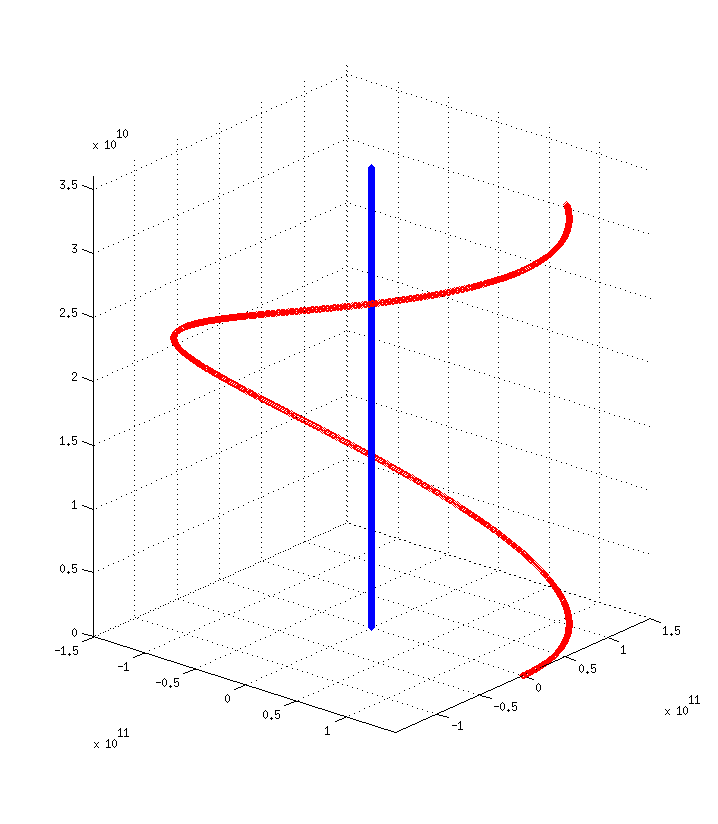
\includegraphics[width=\textwidth]{img/sun_upz_earth_roty}
                \caption{Sun (blue) -- Earth (red)\\With \texttt{input\_sun\_earth.dat}}
                \label{fig:earthsun}
        \end{subfigure}%
        ~ %add desired spacing between images, e. g. ~, \quad, \qquad etc.
          %(or a blank line to force the subfigure onto a new line)
        \begin{subfigure}[b]{0.3\textwidth}
                \centering
                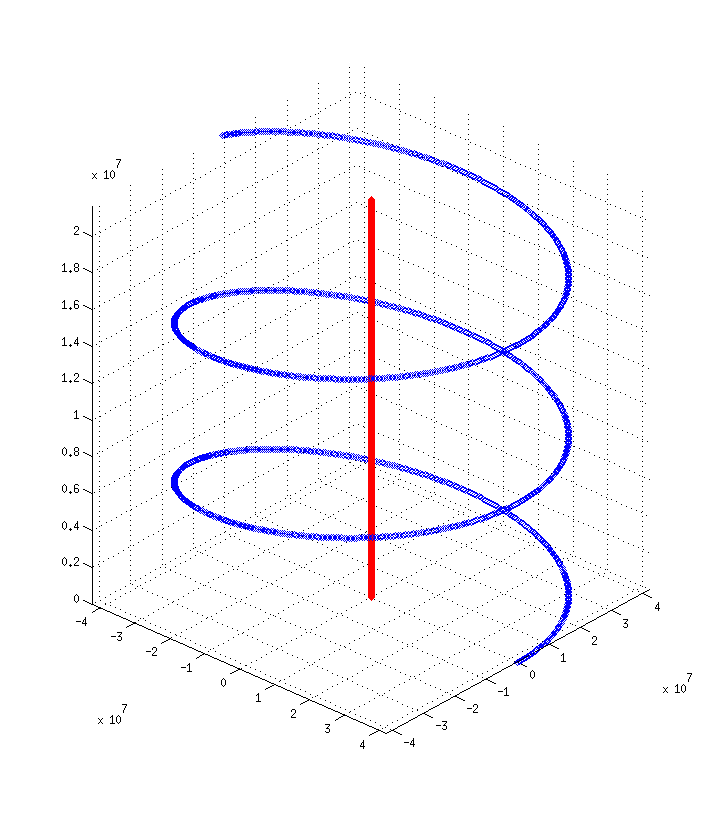
\includegraphics[width=\textwidth]{img/earth_sat}
                \caption{Earth (red) -- Satellite (blue)\\With \texttt{input\_earth\_sat.dat}}
                \label{fig:satgeo}
        \end{subfigure}
        \begin{subfigure}[b]{0.3\textwidth}
                \centering
                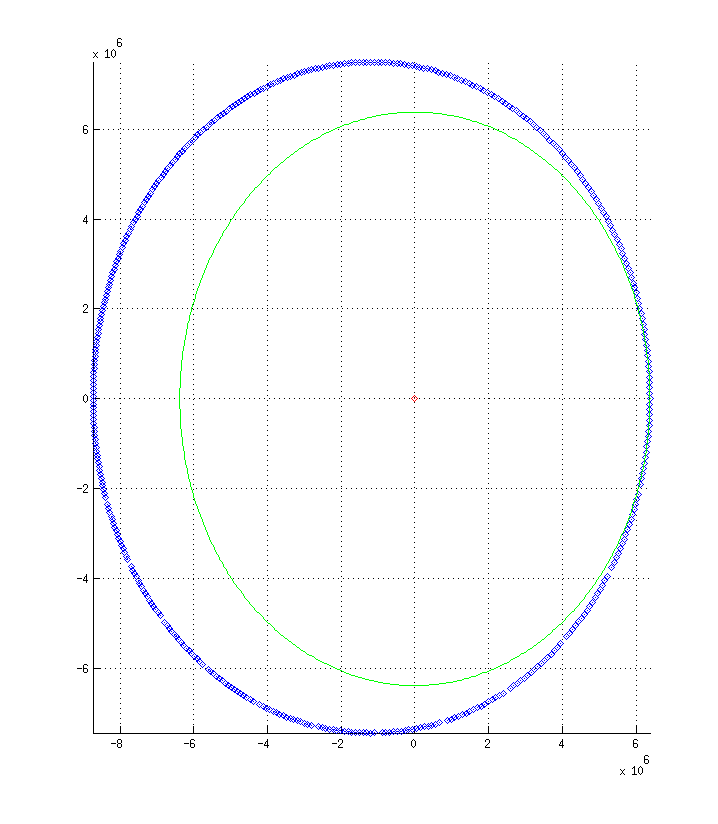
\includegraphics[width=\textwidth]{img/nc}
                \caption{Surface (green) -- Projectile (blue)\\With \texttt{input\_newtons\_cannon.dat}}
                \label{fig:nc}
        \end{subfigure}
        \caption{Orbits around a significant mass. Note the scale difference.\\Newton's Cannon from the Earth's surface.}\label{fig:orbits}
\end{figure}

\begin{figure}[H]
        \centering
%         \hspace{-0.5cm}
        \begin{subfigure}[b]{0.3\textwidth}
                \centering
                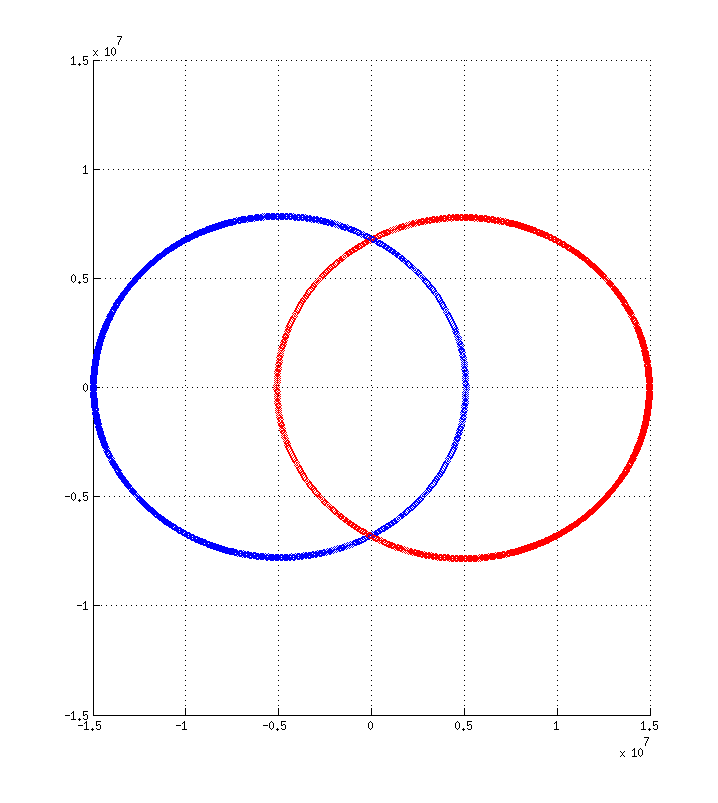
\includegraphics[width=\textwidth]{img/binary_xy}
                \caption{Two-body problem (2D)}
                \label{fig:bin}
        \end{subfigure}%
        ~ %add desired spacing between images, e. g. ~, \quad, \qquad etc.
          %(or a blank line to force the subfigure onto a new line)
        \begin{subfigure}[b]{0.3\textwidth}
                \centering
                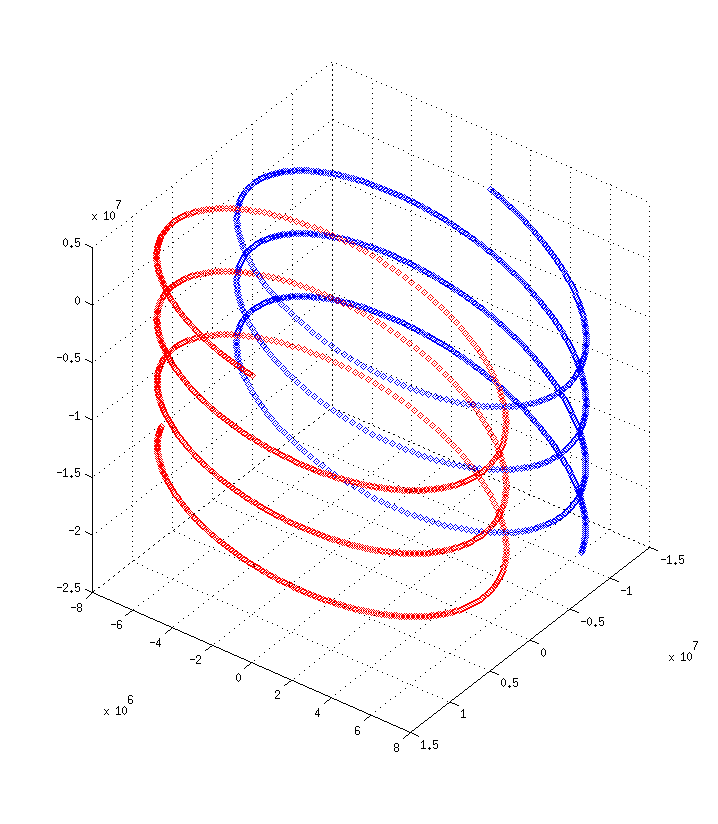
\includegraphics[width=\textwidth]{img/binar_3d}
                \caption{Two-body problem (3D)}
                \label{fig:bin3D}
        \end{subfigure}
        \caption{The two-body symmetric problem. Barycenter is at (0,0).\\With \texttt{input\_two\_body\_problem.dat}}\label{fig:twobody}
\end{figure}

\begin{figure}[H]
        \centering
%         \hspace{-0.5cm}
        \begin{subfigure}[b]{0.7\textwidth}
                \centering
                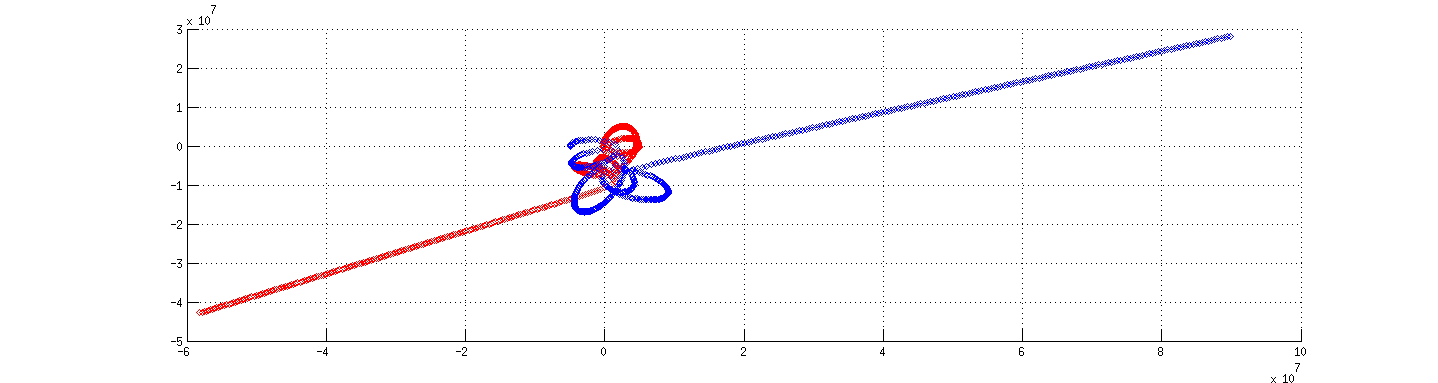
\includegraphics[width=\textwidth]{img/g_k}
                \caption{Bad sampling}
                \label{fig:gk}
        \end{subfigure}%
        ~ %add desired spacing between images, e. g. ~, \quad, \qquad etc.
          %(or a blank line to force the subfigure onto a new line)
        \begin{subfigure}[b]{0.25\textwidth}
                \centering
                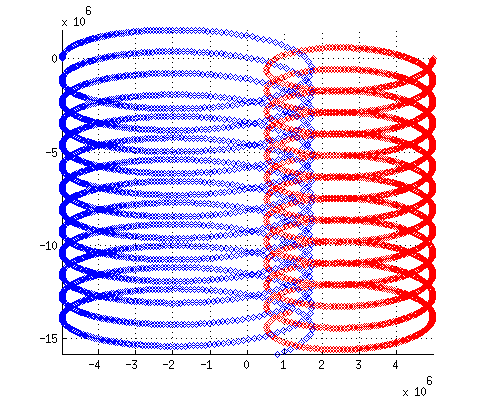
\includegraphics[width=\textwidth]{img/g_k_balanced}
                \caption{Good sampling}
                \label{fig:gkfixed}
        \end{subfigure}
        \caption{Unbalanced two-body problem with and without sampling problem.}\label{fig:sample}
\end{figure}

%\begin{figure}[H]
%  \centering
%  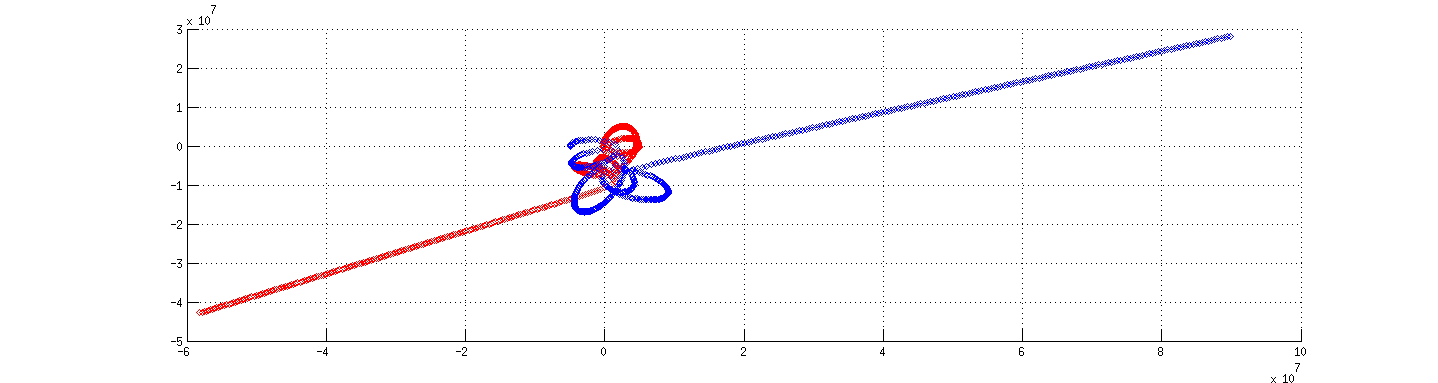
\includegraphics[width=1\textwidth]{img/g_k}
%  \caption{Two-body problem thrown out of balance by bad sampling.}\label{fig:gk}
%\end{figure}

%\begin{table}[H]
%\begin{center}
%\rowcolors{2}{light-gray}{medium-gray}
%\begin{tabular}{| c c c c | c c c c |}
%\hline
%\multicolumn{4}{| c |}{\cellcolor{extra-gray}Internal} & \multicolumn{4}{ c |}{\cellcolor{extra-gray}External} \\ \hline 
%\cellcolor{extra-gray} Source &\cellcolor{extra-gray} Port &\cellcolor{extra-gray} Dest. &\cellcolor{extra-gray} Port &\cellcolor{extra-gray} Source &\cellcolor{extra-gray} Port &\cellcolor{extra-gray} Dest. &\cellcolor{extra-gray} Port \\ \hline \hline \showrowcolors
%192.168.10.1 & 3001 & 128.178.52.93 & 80 & 193.49.96.60 & 3001 & 128.178.50.93 & 80 \\
%192.168.10.2 & 3001 & 128.178.52.93 & 80 & 193.49.96.61 & 3001 & 128.178.50.93 & 80 \\
%192.168.10.3 & 3001 & 128.178.52.93 & 80 & 193.49.96.62 & 3001 & 128.178.50.93 & 80 \\
%192.168.10.4 & 3001 & 128.178.52.93 & 80 & 193.49.96.60 & 3002 & 128.178.50.93 & 80 \\ \hline
%\end{tabular}
%\end{center}
%\end{table}

%\begin{figure}[H]
%  \centering
%  \includegraphics[width=1\textwidth]{Diag.png}
%\end{figure}

\end{document}
